\subsection{Generating Unit-Level Assertions} \label{Sec:unitLevelAssertion}
Our approach targets postcondition assertions which are used to examine the expected behaviour of a given function after it is executed in a unit test case.
By analyzing a given DOM-based test case, we generate unit-level assertions in the following three categories: (1) explicit assertions, (2) implicit assertions, and (3) candidate assertions. 
%Each assertion is coupled with the expected value obtained from the execution trace of the application. The first type of assertion (type 1), which we call explicit assertion, can potentially be used in unit testing of the current version of the application. Type 2 and type 3, which we call implicit assertions and candidate assertions respectively, can be used for the purpose of regression testing.
\subsubsection{Explicit Assertions} \label{Sec:explicitAssertions}
After collecting all the statements, that are relevant to a given DOM-based assertion, we extract accessible entities from these statements (\textsc{Accessibles} in line 23 of the algorithm).
Types of accessible entities include (1) the function's returned value, (2) the used global variables in that function, (3) the object's property where the object is accessible in the outer scope of the function, and/or (4) the accessed DOM element in that function. Dynamic backward slice of a DOM-based assertion helps to (1) track all statements that contribute to the checked result and as such identify those entities that might have influenced the checked property value of the DOM element, and (2) eliminate unrelated entities that are not involved in the computation that leads to the update performed on the checked DOM element.

Since our dynamic slice is extracted from the program run, we can track all concrete values associated with accessible entities.
During the run of a test case, there might be different instances where a given statement is executed. Different execution instances can lead to different behaviour. Since we are using dynamic slicing, an instance that leads to the required behaviour, which is checked through the DOM-based assertion, is on the backward slice. Given that the manually-written expected value, that is checked against the DOM's property is valid, the concrete values of related entities in the backward slice are potentially correct. Therefore, concrete value of an entity in the backward slice can be used as the expected value of the entity in unit-level assertions to test the current version of the application (discussed in \secref{discussion}).
$explicitAsstn$ in line 23 of \algref{algorithm} contains the inferred explicit assertions.

In our running example (\figref{intraCodeDep}), explicit assertions check the correctness of \code{customer.payable}, \code{coupon.expired}, as well as \code{price} and \code{quantity} properties which belong to \code{selItem} object.
Assuming that the original price of the item is 100, the number of selected item is 1, and the calculated discount according to the \code{value} attribute of a DOM element with ID \code{couponButt} is 30, then the expected values included in the assertions for each of the entities are 70, boolean value \code{true}, 100, and 1, respectively. \figref{unitTest} shows a unit test case for \code{addToCart} function with the generated assertions in \qunit framework. %\karthik{What's a \qunit test?} 
Lines 7 to 9 in the figure corresponds to the explicit assertions.
\begin{figure}
  \centering
  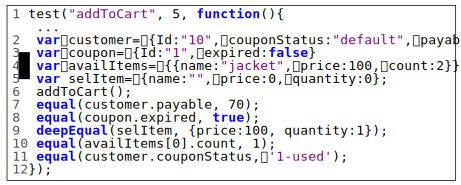
\includegraphics[width=1\hsize]{fig/unitTest}
   \vspace{-0.3in} 
  \mycaption{Generated \qunit test case and assertions.}
  \label{Fig:unitTest}
  \vspace{-0.28in} 
\end{figure}  
%We compare the value of the entity immediately after the relevant statement is executed in the backward slice with the entity's value before the function exits. If value of the entity remains the same, we use it towards the expected value in the unit-level assertion.  
%However, if the entity pertaining to a DOM change is reassigned in the code after the DOM gets updated and before the function exits, then the concrete value of the entity can be used for the purpose of regression testing unless the tester provides the proper expected value.
\subsubsection{Implicit Assertions} \label{Sec:implicitAssertions}
To this end we gather all the statements that explicitly affect the computations relevant to a given DOM-based assertion. While assertions inferred from such statements are inherently important, we further need to consider entities that are implicitly influenced by the checked DOM element in the manually-written test suite. For this purpose we apply a dynamic forward slice on the statements collected from a backward slice of a DOM-based assertion. A forward slice with respect to a statement $st$,
indicates how subsequently an operand at $st$ is being used. This can help the tester to ensure that $st$ properly establishes the expected outcome of the computations assumed by the later statements. 
Given the importance of statements involved in code-level computations of a DOM-based assertion, using forward slice is useful to check that there are no unforeseen effects on the application's behavior by a modification to such statements. 

Dynamic forward slice is performed on the subset of code statements which is previously instrumented as explained in \secref{domToCode}. The process of forwards slicing is similar to the backwards slicing technique as discussed earlier (\secref{domToCode}). The only difference is that it is performed in a forward direction. The slicing criterion of the forward slice module is either a variable, object's property, or an accessed DOM property extracted from the statements in a backward slice. The accessible entities, which have been set within the collected forward slice statements establish our implicit assertions.   
\subsubsection{Candidate Assertions} \label{Sec:candidateAssertions}
In addition to explicit and implicit assertions, we also verify the correctness of code-level entities pertaining to DOM updates, which are essentially important but not checked in the existing DOM-based test cases. We derive such unit-level assertions, namely candidate assertions, from the candidate DOM element properties previously obtained from the test case execution (box 3 in \figref{approachDiagram}). As the test case runs, we monitor DOM's evolution and match the list of mutated DOM elements and their properties with property updates of the candidate DOM elements. Once a match is found, we infer backwards slice statements pertaining to the mutation of DOM element's property (\textsc{GetBWSlice} in line 18 of the algorithm). Therefore, in this case the slicing criteria which is given as input to the backwards slicing module is an update to the property of the candidate DOM element.
After gathering the related \javascript statements within the application, we extract accessible entities of these statements (\textsc{Accessibles} in line 22) which form our candidate assertions. $candidateAsstn$ in line 22 contains our candidate assertions. 

Recall from the example (\figref{example}), one such potential DOM property which we record as part of \secref{extractDomRelatedInfo}, is \code{class} attribute associated with DOM element with ID \code{couponButt}. Monitoring DOM changes reveal that line 26, where the \code{class} attribute of the element is set, is the initial point of contact between DOM mutation and the \javascript code. Given line 26 as the slicing criteria, \code{customer.couponStatus} (line 24) is marked as the candidate assertion.
 